\documentclass[10pt,a4paper]{article}
\usepackage[margin=2cm]{geometry}
\usepackage[T1]{fontenc}
\usepackage{lmodern}
\usepackage{amsmath,amssymb}
\usepackage{booktabs,array,tabularx}
\usepackage{enumitem}
\usepackage[dvipsnames]{xcolor}
\usepackage{tikz}
\usetikzlibrary{arrows.meta,positioning,calc,fit,backgrounds}
\usepackage[most]{tcolorbox}
\usepackage[colorlinks=true,linkcolor=blue!60!black,urlcolor=blue!60!black]{hyperref}

\setlist{nosep,leftmargin=1.2em}
\setlength{\parindent}{0pt}
\setlength{\parskip}{4pt}

\newcommand{\code}[1]{\texttt{\detokenize{#1}}}
\newtcolorbox{keybox}[1]{colback=blue!3,colframe=blue!45!black,fonttitle=\bfseries,title=#1,boxrule=0.6pt,arc=1mm,left=4pt,right=4pt,top=2pt,bottom=2pt}
\newtcolorbox{notebox}{colback=orange!5,colframe=orange!70!black,boxrule=0.6pt,arc=1mm,left=4pt,right=4pt,top=2pt,bottom=2pt}

\tikzset{
  blk/.style={draw,thick,minimum height=8mm,minimum width=12mm,align=center,fill=white,font=\small},
  sum/.style={draw,thick,circle,minimum size=5mm,inner sep=0pt,fill=white},
  sig/.style={-{Latex[length=2mm]},thick},
  lbl/.style={font=\scriptsize},
  plant/.style={blk,fill=green!6},
  ctrl/.style={blk,fill=blue!5},
  ffb/.style={blk,fill=orange!10},
}

\title{\textbf{Pole placement for the CNC plotter}\\[2pt]
\large design guide: workflow, design A and its parameters, feedforward fit}
\author{scripts: \code{scripts/control/pp_design}, \code{scripts/control/ff_correct.m}}
\date{}

\begin{document}
\maketitle
\vspace{-6mm}

\begin{keybox}{What this document covers}
\begin{enumerate}
  \item \textbf{The workflow in short} (Sec.~\ref{sec:workflow}): which script does what, including the tools for
        tuning by hand (\code{design_B}, \code{check_design}, \code{tune_poles}, \code{explore_poles}).
  \item \textbf{Plant and controller} (Sec.~\ref{sec:plant}--\ref{sec:ctrl}): the simulated motor with friction and
        delay, the control law and its block diagram.
  \item \textbf{Design A} (Sec.~\ref{sec:designA}--\ref{sec:result}), the core of the method: pole pattern, gains,
        every parameter and requirement with its justification, the search and the final numbers.
  \item \textbf{Feedforward fit} (Sec.~\ref{sec:ff}): how the feedforward is corrected from a run, for any controller.
\end{enumerate}
\end{keybox}

%==========================================================================================
\section{The workflow at a glance}\label{sec:workflow}

\begin{center}
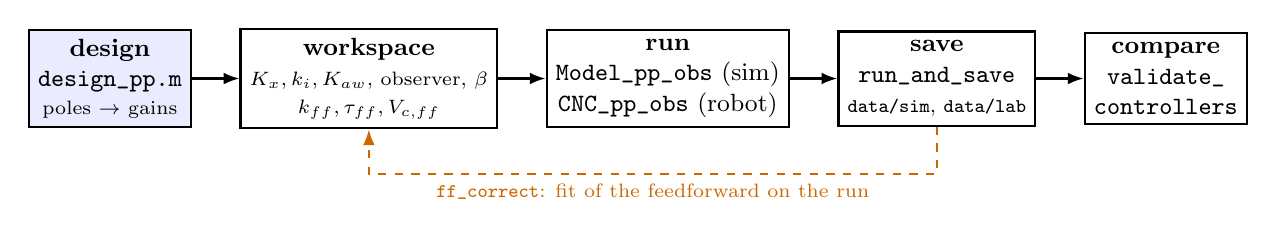
\begin{tikzpicture}[node distance=7mm and 6mm]
  \node[blk,fill=blue!8] (des) {\textbf{design}\\ \code{design_pp.m}\\[-1pt]\scriptsize poles $\to$ gains};
  \node[blk,right=of des] (ws) {\textbf{workspace}\\ \scriptsize $K_x,k_i,K_{aw}$, observer, $\beta$\\[-1pt]\scriptsize $k_{ff},\tau_{ff},V_{c,ff}$};
  \node[blk,right=of ws] (sim) {\textbf{run}\\ \code{Model_pp_obs} (sim)\\ \code{CNC_pp_obs} (robot)};
  \node[blk,right=of sim] (save) {\textbf{save}\\ \code{run_and_save}\\ \scriptsize\code{data/sim}, \code{data/lab}};
  \node[blk,right=of save] (cmp) {\textbf{compare}\\ \code{validate_}\\ \code{controllers}};
  \draw[sig] (des) -- (ws); \draw[sig] (ws) -- (sim); \draw[sig] (sim) -- (save); \draw[sig] (save) -- (cmp);
  \draw[sig,dashed,orange!80!black] (save.south) |- ++(0,-6mm) -| node[lbl,pos=0.25,below]{\code{ff_correct}: fit of the feedforward on the run} (ws.south);
\end{tikzpicture}
\end{center}

\textbf{Steps.}
\begin{enumerate}
  \item Set the requirements once in \code{utils/pp_setup.m} (Sec.~\ref{sec:req}); they hold for every design.
  \item Run \code{design_pp.m}: it searches the poles of design A, prints the requirement table, plots the
        steps and writes the gains to the workspace.
  \item In the same script, \code{ff_source} decides the feedforward: \code{'model'} (no fit), \code{'sim'} (one
        simulation, fit, final simulation) or \code{'run'} (fit on a saved run, e.g.\ from the robot).
  \item Compare runs with \code{validate_controllers.m} (contour error, tracking error, voltage, margins).
\end{enumerate}

\textbf{The other scripts} (folder \code{tools/}: exploration and tuning by hand; same gains, observer and requirements):

\begin{tabularx}{\linewidth}{@{}l X@{}}
\toprule
script & use \\
\midrule
\code{design_pp.m} & \textbf{main script}: design A + search + feedforward correction + final run \\
\code{design_B.m} & three real poles $-\lambda_1,-\lambda_2,-\lambda_3$, each moved on its own by the search. No
  oscillating mode but a slower rise; it served as a step towards design A and is kept for comparison \\
\code{check_design.m} & poles given by hand (pattern A or the three poles per motor), no search: only checks and
  writes them \\
\code{tune_poles.m} & sliders for $\omega_n,\zeta,\alpha$ on both motors; \emph{lock alpha} keeps the integral pole fixed \\
\code{explore_poles.m} & drag the three poles of one motor and watch step, voltage and Bode live \\
\code{utils/} & \code{pp_setup} (models, requirements), \code{pp_gains} (poles $\to$ gains, observer),
  \code{closed_loop} (simulation with delay), \code{pp_check}, \code{pp_search}, \code{pp_report},
  \code{pp_simulink} (workspace variables) \\
\code{../ff_correct.m} & feedforward fit, shared with the PID (Sec.~\ref{sec:ff}) \\
\bottomrule
\end{tabularx}

%==========================================================================================
\section{Plant model and simulated plant}\label{sec:plant}

\textbf{Model used by the controller} (one per joint, identified with the linkage attached, angle in encoder degrees):
\begin{equation}
  \tau\ddot\theta + \dot\theta = b\,u,\qquad G(s)=\frac{b}{s(\tau s+1)},\qquad b=-\frac{180}{\pi}k,
\end{equation}
\begin{equation}
  x=\begin{bmatrix}\theta\\ \omega\end{bmatrix},\quad
  A=\begin{bmatrix}0&1\\0&-1/\tau\end{bmatrix},\quad
  B=\begin{bmatrix}0\\ b/\tau\end{bmatrix},\quad
  C=\begin{bmatrix}1&0\end{bmatrix}.
\end{equation}
$k,\tau$ = \code{k_xxxx_load}, \code{tau_xxxx_load} ($k\approx1.44/1.38$~rad/(V\,s), $\tau\approx0.037$~s, so the mechanical
pole is $1/\tau\approx27$~rad/s). The minus sign in $b$ is the encoder convention (a positive voltage gives a negative angle).

\textbf{Simulated plant} (\code{motor model xxxx} in the \code{Model_*} files). To test the controller against a plant
that is \emph{not} its model, \code{parameters.m} (section 5) provides a ``realistic'' plant from the multisine fit with
delay and Coulomb friction:
\begin{equation}
  u_m(t) = u_{sat}(t-T_d) - V_c\tanh\!\left(\frac{\omega_m}{w_\varepsilon}\right),\qquad
  \omega_m = \frac{k_p}{\tau_p s+1}\,u_m,\qquad \theta = -\frac{180}{\pi}\int\omega_m\,dt .
\end{equation}

\begin{center}
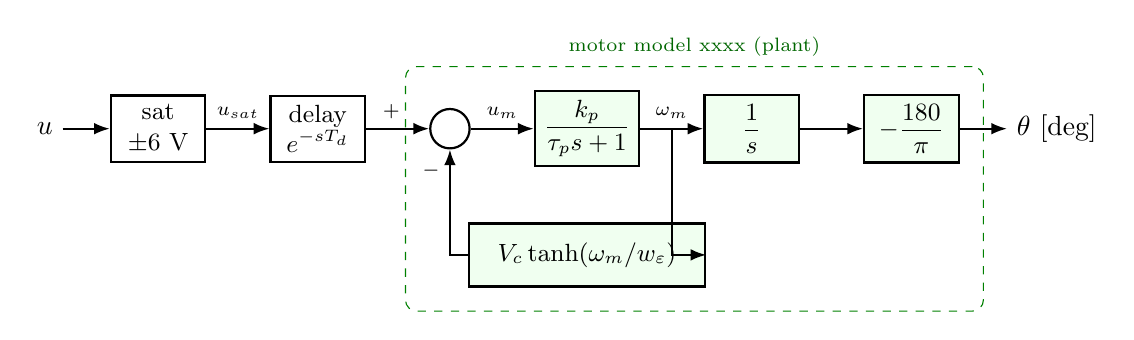
\begin{tikzpicture}[node distance=6mm and 8mm]
  \node (in) {$u$};
  \node[blk,right=6mm of in] (sat) {sat\\ $\pm6$ V};
  \node[blk,right=of sat] (del) {delay\\ $e^{-sT_d}$};
  \node[sum,right=of del] (s1) {};
  \node[plant,right=of s1] (tf) {$\dfrac{k_p}{\tau_p s+1}$};
  \node[plant,right=of tf] (int) {$\dfrac1s$};
  \node[plant,right=of int] (g) {$-\dfrac{180}{\pi}$};
  \node[right=6mm of g] (out) {$\theta$ [deg]};
  \node[plant,below=7mm of tf,minimum width=30mm] (fr) {$V_c\tanh(\omega_m/w_\varepsilon)$};
  \draw[sig] (in) -- (sat); \draw[sig] (sat) -- node[lbl,above]{$u_{sat}$} (del);
  \draw[sig] (del) -- node[lbl,above,pos=0.4]{$+$} (s1);
  \draw[sig] (s1) -- node[lbl,above]{$u_m$} (tf);
  \draw[sig] (tf) -- node[lbl,above]{$\omega_m$} coordinate[midway](om) (int);
  \draw[sig] (int) -- (g); \draw[sig] (g) -- (out);
  \draw[sig] (om) |- (fr.east);
  \draw[sig] (fr.west) -| node[lbl,left,pos=0.9]{$-$} (s1.south);
  \begin{scope}[on background layer]
    \node[draw,dashed,green!50!black,rounded corners,fit=(s1)(tf)(int)(g)(fr),inner sep=3mm,
          label={[lbl,green!40!black]above:motor model xxxx (plant)}] {};
  \end{scope}
\end{tikzpicture}
\end{center}

\begin{tabularx}{\linewidth}{@{}l c c X@{}}
\toprule
\code{use_real_plant} & $k_p,\ \tau_p$ & $T_d,\ V_c$ & meaning \\
\midrule
\code{false} & $k,\ \tau$ (= model) & 0, 0 & plant = model: checks the design itself \\
\code{true}  & 1.77/1.74,\ 0.043/0.044 s & 3.5 ms,\ 0.12/0.14 V & plant $\neq$ model, as on the bench \\
\bottomrule
\end{tabularx}

\begin{notebox}
\textbf{Where friction and delay live.} Friction and $k_p,\tau_p$ belong to the \emph{plant} (motor model subsystem):
the friction depends on the real speed $\omega_m$ and opposes it. The block computing $V_c\tanh(\cdot)$ uses the output of the
strictly proper block $k_p/(\tau_p s+1)$, so there is no algebraic loop. \code{scripts/update_models.m} adds them to
\code{Model_pp_obs} and \code{Model_pid_ff}. The delay $T_d$ belongs to the plant too and must not be copied into the
\code{CNC_*} models, where the real motor provides it.
\end{notebox}

%==========================================================================================
\section{Control law and controller block}\label{sec:ctrl}

Only $\theta$ is measured: a Luenberger observer gives $\hat x=[\hat\theta,\hat\omega]^T$. With the reference
$\phi$ (degrees) and its derivatives $\dot\phi,\ddot\phi$ (rad/s, rad/s$^2$) from the inverse kinematics:
\begin{equation}\label{eq:law}
  u = \underbrace{-K_x\left(\hat x - x_{ref}\right)}_{\text{state feedback}}
      \;\underbrace{-\,k_i e_I}_{\text{integral}}
      \;\underbrace{-\frac{1}{k_{ff}}\dot\phi - \frac{\tau_{ff}}{k_{ff}}\ddot\phi}_{\text{feedforward}}
      \;\underbrace{-\,V_{c,ff}\tanh\!\left(\frac{\dot\phi}{w_\varepsilon}\right)}_{\text{friction compensation}},
  \qquad x_{ref}=\begin{bmatrix}\beta\phi\\ \tfrac{180}{\pi}\dot\phi\end{bmatrix},
\end{equation}
\begin{equation}
  \dot e_I = \phi - y + K_{aw}(u_{sat}-u),\qquad
  \dot{\hat x} = A_{obs}\hat x + B_{obs}\begin{bmatrix}u_{sat}\\ y\end{bmatrix},\quad A_{obs}=A-LC,\ B_{obs}=[B\ \ L].
\end{equation}

\begin{center}
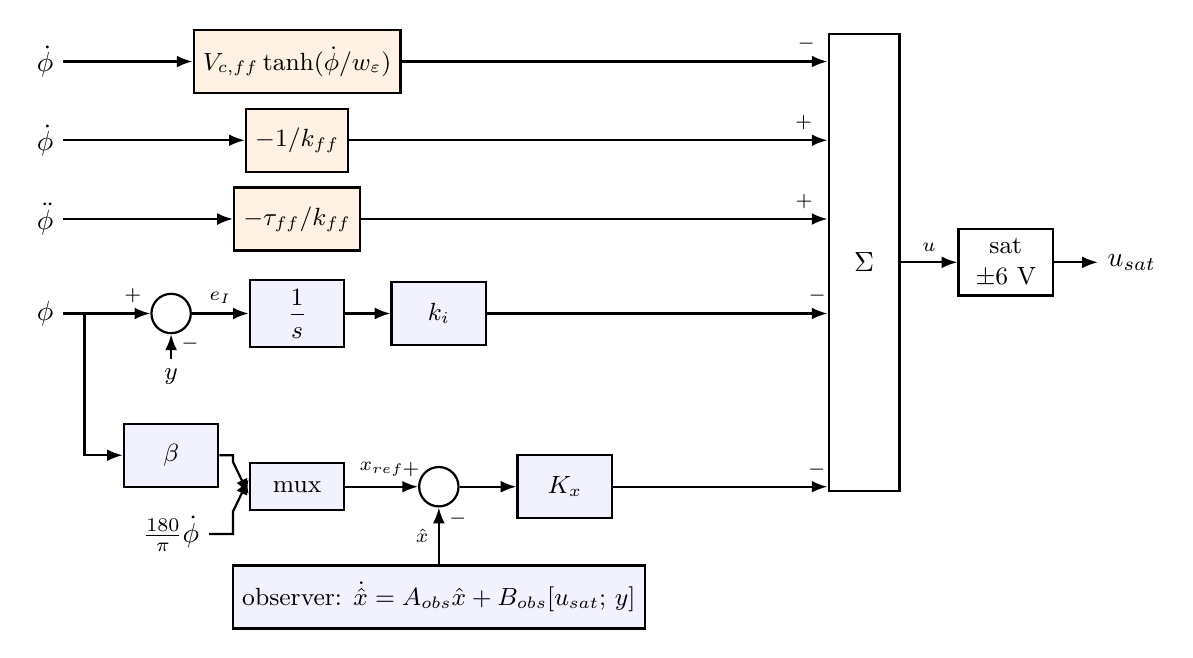
\begin{tikzpicture}
  % big summing block: every branch enters from the left with its sign
  \node[draw,thick,minimum width=9mm,minimum height=58mm,fill=white] (su) at (10.4,-0.35) {$\Sigma$};
  % feedforward rows (orange, outside the loop)
  \node (dphi0) at (0,2.2) {$\dot\phi$};
  \node[ffb] (fc) at (3.2,2.2) {$V_{c,ff}\tanh(\dot\phi/w_\varepsilon)$};
  \node (dphi1) at (0,1.2) {$\dot\phi$};
  \node[ffb] (kv) at (3.2,1.2) {$-1/k_{ff}$};
  \node (ddphi) at (0,0.2) {$\ddot\phi$};
  \node[ffb] (ka) at (3.2,0.2) {$-\tau_{ff}/k_{ff}$};
  % integral row
  \node (phi) at (0,-1.0) {$\phi$};
  \node[sum] (se) at (1.6,-1.0) {};
  \node[ctrl] (int) at (3.2,-1.0) {$\dfrac1s$};
  \node[ctrl] (ki) at (5.0,-1.0) {$k_i$};
  \node (yin) at (1.6,-1.8) {\small $y$};
  % state feedback row
  \node[ctrl] (beta) at (1.6,-2.8) {$\beta$};
  \node (dref) at (1.6,-3.8) {$\tfrac{180}{\pi}\dot\phi$};
  \node[ctrl,minimum height=6mm] (mux) at (3.2,-3.2) {mux};
  \node[sum] (sx) at (5.0,-3.2) {};
  \node[ctrl] (kx) at (6.6,-3.2) {$K_x$};
  \node[ctrl] (obs) at (5.0,-4.6) {observer: $\dot{\hat x}=A_{obs}\hat x+B_{obs}[u_{sat};\,y]$};
  % output
  \node[blk] (sat) at (12.2,-0.35) {sat\\ $\pm6$ V};
  \node (u) at (13.8,-0.35) {$u_{sat}$};
  % wires
  \draw[sig] (dphi0) -- (fc);  \draw[sig] (fc.east)  -- node[lbl,above,pos=0.95]{$-$} (fc.east -| su.west);
  \draw[sig] (dphi1) -- (kv);  \draw[sig] (kv.east)  -- node[lbl,above,pos=0.95]{$+$} (kv.east -| su.west);
  \draw[sig] (ddphi) -- (ka);  \draw[sig] (ka.east)  -- node[lbl,above,pos=0.95]{$+$} (ka.east -| su.west);
  \draw[sig] (phi) -- node[lbl,above,pos=0.8]{$+$} (se);
  \draw[sig] (yin) -- node[lbl,right,pos=0.6]{$-$} (se);
  \draw[sig] (se) -- node[lbl,above]{$e_I$} (int);
  \draw[sig] (int) -- (ki);
  \draw[sig] (ki.east) -- node[lbl,above,pos=0.97]{$-$} (ki.east -| su.west);
  \draw[sig] (0.5,-1.0) |- (beta.west);
  \draw[sig] (beta.east) -| ([xshift=-2mm]mux.north west) -- ([yshift=-1mm]mux.north west |- mux.west);
  \draw[sig] (dref.east) -| ([xshift=-2mm]mux.south west) -- ([yshift=1mm]mux.south west |- mux.west);
  \draw[sig] (mux) -- node[lbl,above]{$x_{ref}$} node[lbl,above,pos=0.9]{$+$} (sx);
  \draw[sig] (obs.north) -- node[lbl,left,pos=0.5]{$\hat x$} node[lbl,right,pos=0.8]{$-$} (sx);
  \draw[sig] (sx) -- (kx);
  \draw[sig] (kx.east) -- node[lbl,above,pos=0.95]{$-$} (kx.east -| su.west);
  \draw[sig] (su) -- node[lbl,above]{$u$} (sat);
  \draw[sig] (sat) -- (u);
\end{tikzpicture}
\end{center}
Blocks in orange: the feedforward, outside the loop; blue: the loop designed by pole placement. Not drawn: the
anti-windup term $K_{aw}(u_{sat}-u)$, added to the input of the integrator. The same structure is in
\code{pp + luenberg xxxx} of \code{Model_pp_obs} and \code{CNC_pp_obs}; the PID models have the same orange branch.

\begin{tabularx}{\linewidth}{@{}l X@{}}
\toprule
block & role \\
\midrule
feedforward & the voltage the nominal motor needs to follow $\dot\phi,\ddot\phi$: the feedback only corrects errors \\
friction comp. & $V_{c,ff}\tanh(\dot\phi/w_\varepsilon)$ from the \emph{reference} speed; $\tanh$ instead of $\mathrm{sign}$ avoids a voltage jump at zero speed \\
integral $k_i$ & removes constant errors (friction, load, errors in $k$); $K_{aw}=-\overline{|p|}/k_i$ unloads it when the amplifier saturates \\
$K_x$, $\beta$ & state feedback on $\hat x-x_{ref}$; $\beta$ weights the position reference (Sec.~\ref{sec:beta}) \\
observer & estimates $\omega$ from $\theta$ and the voltage really applied ($u_{sat}$) \\
\bottomrule
\end{tabularx}

%==========================================================================================
\section{Design A: pole pattern and gains}\label{sec:designA}

With $\hat x=x$ and states $z=[\theta,\omega,e_I]^T$, the loop is $\dot z=(A_i-B_iK)z$ with
$A_i=\begin{bmatrix}A&0\\-C&0\end{bmatrix}$, $B_i=\begin{bmatrix}B\\0\end{bmatrix}$, $K=[k_1\ k_2\ k_i]$.
Its characteristic polynomial and the gains that place the poles (polynomial matching, \code{acker} gives the same):
\begin{equation}
  \Delta(s)=s^3+a_2s^2+a_1s+a_0,\qquad
  a_2=\frac{1+bk_2}{\tau},\quad a_1=\frac{bk_1}{\tau},\quad a_0=-\frac{bk_i}{\tau},
\end{equation}
\begin{equation}\label{eq:gains}
  k_1=\frac{\tau a_1}{b},\qquad k_2=\frac{\tau a_2-1}{b},\qquad k_i=-\frac{\tau a_0}{b},\qquad
  \Delta(s)=(s-p_1)(s-p_2)(s-p_3).
\end{equation}
Each gain appears in one coefficient only: for any choice of poles the gains exist and are unique (the pair $(A_i,B_i)$ is
reachable).

\textbf{Design A} writes the three poles as a complex pair and a real pole:
\begin{equation}
  p_{1,2}=-\zeta\omega_n\pm j\omega_n\sqrt{1-\zeta^2},\qquad p_3=-\lambda=-\alpha\zeta\omega_n .
\end{equation}
Three numbers with a physical meaning instead of three free poles: the pair sets speed and damping of the joint, the real pole
the integral action. From \eqref{eq:gains}, with $a_1=\omega_n^2+2\zeta\omega_n\lambda$ and $a_0=\omega_n^2\lambda$:
\begin{equation}\label{eq:approx}
  |k_1|\approx\frac{\tau\,\omega_n^2}{|b|}\quad\text{[V/deg]},\qquad
  |k_i|=\frac{\tau\,\omega_n^2\lambda}{|b|}\quad\text{[V/(deg\,s)]}.
\end{equation}

\textbf{Observer.} Poles $-o_1,-o_2$ with $o_1=\min(6\max|p_i|,\,250)$, $o_2=1.25\,o_1$;
$L$ = \code{acker(A', C', p_obs)'}. By separation the estimation error obeys $\dot\varepsilon=(A-LC)\varepsilon$: the observer
does not move the three controller poles.

%==========================================================================================
\section{Every parameter and why it has this value}\label{sec:params}

\subsection{Pole parameters (section 1 of \texttt{design\_pp.m})}

\begin{tabularx}{\linewidth}{@{}l c X@{}}
\toprule
parameter & start value & justification \\
\midrule
$\omega_n$ & 45 rad/s &
  Speed and stiffness of the joint. A model error $\Delta u$ (friction, wrong $k$) gives an angle error
  $e\approx\Delta u/|k_1|$ with $|k_1|\propto\omega_n^2$: faster is better for tracking. Upper limits: phase lost in the
  delay ($\omega_cT_d$), encoder noise on $u$ (chatter), observer at most 250 rad/s. 45 is a deliberately high start: the
  search lowers it until the limits are met (Sec.~\ref{sec:result}). \\
$\zeta$ & 0.9 &
  Damping of the pair. Low $\zeta$ $\Rightarrow$ ringing at the corners and a large $M_s$; with the delay, the margin
  requirements push $\zeta$ towards 1. Capped at 0.999 so that the pair stays complex (pattern A). \\
$\lambda=\alpha\zeta\omega_n$ & 12 rad/s &
  Speed of the integral action: a residual error decays as $e^{-\lambda t}$ (gone in $4/\lambda$). The fundamental of the
  path is $2\pi/T=1.6$ rad/s with $T=4$ s: the error from model mismatch is attenuated by $|GS|\approx1/|k_i|\propto
  1/\lambda$, so a faster $\lambda$ is cheap in voltage. Too close to the pair it removes phase at crossover
  (rule $\lambda\lesssim0.3\,\zeta\omega_n$). \\
\code{beta_mode} & \code{'one'} &
  $\beta=1$ for trajectories (Sec.~\ref{sec:beta}). \\
\code{start_from_pid} & \code{false} &
  The search stays as close as possible to the start; starting from the PID poles would return a controller as slow as the
  PID. \\
\code{do_search} & \code{true} &
  Corrects only what violates a requirement, starting from the values above. \\
\bottomrule
\end{tabularx}

\subsection{The reference weight $\beta$}\label{sec:beta}
$\beta$ is outside the loop: it changes the zero of the reference-to-angle transfer, not the poles, margins or load response:
\begin{equation}
  \frac{\Theta(s)}{R(s)}=\frac{\beta a_1 s+a_0}{\Delta(s)},\qquad z=-\frac{a_0}{\beta a_1},\qquad \frac{\Theta(0)}{R(0)}=1 .
\end{equation}
\begin{itemize}
  \item $\beta=1$: on a path the feedback acts on $\theta-\phi$, so it does not lag the reference; the step overshoots
        (slow zero) but a step never happens on the path. \textbf{Used for trajectories.}
  \item $\beta^*=a_0/(a_1\lambda)=1/(1+2\alpha\zeta^2)$: the zero cancels the real pole, the step is the classic second
        order $\omega_n^2/(s^2+2\zeta\omega_n s+\omega_n^2)$. Used for point-to-point steps.
  \item $\beta<1$ on a path: the integral must continuously make up $(1-\beta)k_1\phi$, so the error grows.
\end{itemize}

\subsection{Requirements (\texttt{utils/pp\_setup.m})}\label{sec:req}
Every requirement is checked on both motors (the worst counts), on a reference step of $R$ degrees simulated with the
delay $T_d$ (\code{closed_loop.m}).

\begin{tabularx}{\linewidth}{@{}l c X@{}}
\toprule
requirement & value & justification \\
\midrule
$R$ & 3$^\circ$ &
  Size of the test step. On a path the error is a few degrees at most; only the peak-voltage check depends on it
  ($u(0^+)=k_1R$ with $\beta=1$). Overshoot and settling are switched off with $\beta=1$. \\
peak voltage & 6 V & real saturation of the amplifier: the linear design stays valid. \\
phase margin & $\geq45^\circ$ & robustness to delay and to errors in $k,\tau$. \\
$M_s=\max_\omega|1/(1+L)|$ & $\leq1.6$ &
  $1/M_s$ is the distance of the Nyquist curve from $-1$: it guarantees together
  $GM\geq M_s/(M_s-1)=8.5$ dB (a gain error of $\times2.6$, more than the $+23\%$ of the plant) and
  $PM\geq2\arcsin\frac{1}{2M_s}=36^\circ$. \\
chatter & $\leq0.5$ V &
  one encoder count ($q=360/4096^\circ$) times the controller gain above 100 rad/s: the noise on $u$.
  In practice the cap on $\omega_n$ without delay. \\
slowest pole & $\lambda\geq10$ rad/s &
  The integral must remove an error (friction changes sign at every corner) within a side ($T/4=1$ s):
  $4/\lambda\leq T/4\Rightarrow\lambda\geq4$ rad/s; 10 rad/s gives margin and a larger $k_i$. \\
delay $T_d$ & $1.5T_s+3.5$ ms $=6.5$ ms &
  $1.5T_s$: hold ($T_s/2$) + one sample of computation of the 2 ms controller; 3.5 ms: input delay measured in the
  multisine fit. A delay removes phase $\omega T_d$ without changing the gain: it must be in the design, otherwise the
  margins are optimistic (Sec.~\ref{sec:result}). \\
\bottomrule
\end{tabularx}

\subsection{The search}
\code{pp_search.m} minimises with Nelder--Mead (\code{fminsearch}, in logarithms so that every parameter stays positive)
\begin{equation}
  J(x)=\underbrace{\sum_{i=1}^{3}\left(\log|p_i(x)|-\log|p_{i,0}|\right)^2}_{\text{stay close to the start}}
  \;+\;w\underbrace{\sum_{k=1}^{7}\max\left(0,g_k(x)\right)^2}_{\text{violated requirements only}},\qquad w=10^4,
\end{equation}
with $x=[\omega_n,\zeta,\alpha]$ and normalised violations $g=\text{value}/\text{limit}-1$ (upper limits) or
$1-\text{value}/\text{limit}$ (lower limits). The large $w$ means: first meet every requirement, then move as little as
possible. If two requirements conflict the result is the best compromise and the table marks it with \code{*}.

%==========================================================================================
\section{Result and why the search moved the poles}\label{sec:result}

Margins of the loop broken at the motor input (linear model, motor 3165):

\begin{tabularx}{\linewidth}{@{}l l c c c X@{}}
\toprule
poles & loop & $\omega_c$ [rad/s] & PM & $M_s$ & \\
\midrule
start: $\omega_n=45,\ \zeta=0.9,\ \lambda=12$ & model, $T_d=3$ ms & 53 & $49^\circ$ & 1.53 & looks fine with the old delay \\
 & model, $T_d=6.5$ ms & 53 & $39^\circ$ & 1.96 & violates PM and $M_s$ \\
 & plant ($k_p$, $\tau_p$), 6.5 ms & 57 & $34^\circ$ & 2.18 & fragile on the real plant \\
\midrule
\textbf{result}: $\omega_n=31.8,\ \zeta=0.999,\ \lambda=10$ & model, $T_d=6.5$ ms & 35 & $50^\circ$ & 1.59 & meets every requirement \\
 & plant ($k_p$, $\tau_p$), 6.5 ms & 39 & $45^\circ$ & 1.72 & still acceptable \\
\bottomrule
\end{tabularx}

\begin{itemize}
  \item The real delay is what limits the speed: at the start crossover (53 rad/s) 6.5 ms cost $20^\circ$ of phase.
        The search lowers $\omega_n$ until $M_s=1.6$, and $\lambda$ to its minimum (the integral pole adds phase lag near
        crossover).
  \item $\zeta$ goes to the cap 0.999: with a delay, a well damped pair gives the lowest $M_s$ for a given speed. The pair
        is then almost two coincident real poles at $\approx32$ rad/s, which is still pattern A.
  \item Gains: $k_i=4.6/4.9$ (3165/3166), observer poles $-191/-239$ rad/s (6 times the controller, below 250).
\end{itemize}

%==========================================================================================
\section{Feedforward fit}\label{sec:ff}

\textbf{Idea.} The feedforward gives the voltage the motion needs; the feedback supplies only what the feedforward misses,
and it needs an error to do so. If the model behind the feedforward is wrong, an error remains. In the periodic regime the
angle follows the reference ($y\approx\phi$), so the logged controller voltage $u$ is the voltage the \emph{plant} needs to
follow $\phi$, whatever controller produced it. Fitting $u$ on signals built from the reference identifies the inverse model
of the plant:
\begin{equation}
  u \approx c_1\dot\phi + c_2\ddot\phi + c_3\tanh\!\left(\frac{\dot\phi}{w_\varepsilon}\right)
         + c_4 \qquad\text{(least squares on the periodic regime)}.
\end{equation}
Comparing with the feedforward \eqref{eq:law}:
\begin{equation}
  k_{ff}=-\frac{1}{c_1},\qquad \tau_{ff}=\frac{c_2}{c_1},\qquad V_{c,ff}=-c_3 .
\end{equation}
$c_4$ is a constant offset, not used. The code is explained line by line in \code{ff_fit_explained.pdf}.

\textbf{Why it is sound.}
\begin{itemize}
  \item The feedforward is outside the loop: poles, margins and $M_s$ do not change.
  \item The regressors come from the reference, known and noise free, not from the measured $y$: no noise bias in the fit.
  \item $R^2\approx1$ means the residual error was model error and the new feedforward removes it; a low $R^2$ means the rest
        is noise or effects not in the fit (e.g.\ coupling).
  \item Only $\phi$ and $u$ are used: the same function works for pole placement, PID or any other controller with this
        feedforward (\code{scripts/control/ff_correct.m}).
\end{itemize}

\textbf{What it learns.} The fit can only learn what is in the data. In simulation it learns what the simulated plant has in
more than the model ($k_p,\tau_p$, friction, delay: a delay appears as a larger $\tau_{ff}$, since anticipating the voltage by
$T_d$ adds $T_d\ddot\phi$). On the robot it learns the real motor.

\subsection{Which run the fit needs, and how to get it}\label{sec:ffrun}

\textbf{The run is not ``wrong data''.} The fit does not need a good controller or a good feedforward. It needs only:
\begin{itemize}
  \item the angle roughly following the reference ($y\approx\phi$), so that $u$ is the voltage that produces $\phi$;
  \item the logged reference $\phi$ (\code{r_xxxx}) and controller voltage $u$ (\code{u_xxxx}).
\end{itemize}
A run with the model feedforward is exactly such a run: the voltage the feedforward misses is supplied by the feedback,
so the total $u$ still contains what the plant needs. The fit extracts it from there. That run is also the baseline of the
comparison (``PP + FF model'' vs ``PP + FF fit''), so it is needed anyway.

\textbf{Any controller, any earlier run.} The fit identifies the \emph{plant}, not the controller: a run done with the PID,
or with an older pole placement design, is equally good, provided that
\begin{enumerate}
  \item it was done on the same plant (same motors, same linkage and load);
  \item the trajectory covers speeds and accelerations similar to the ones that will be used afterwards (the fit is valid
        in the range it has seen);
  \item \code{t_skip} excludes the start of that run, so only the periodic regime is used.
\end{enumerate}
For old run files without \code{Vc_xxxx_ff} the printed before/after comparison assumes no friction compensation in
that run; the fitted values do not depend on it.

\textbf{In simulation} (\code{ff_source = 'sim'}) the script does everything: it runs the model with the model feedforward,
saves that run, fits, writes the new values and runs the model again. The two saved runs are the ``FF model'' and
``FF fit'' cases. Useful as a rehearsal before the lab: with \code{use_real_plant = true} the fit must recover the simulated
plant ($k\approx1.77$, $\tau\approx0.043$ s, $V_c\approx0.12$ V), which checks the whole procedure.

\textbf{On the robot} the data must come from the robot, because the fit learns the real motor:

\begin{tabularx}{\linewidth}{@{}c l X@{}}
\toprule
step & where & what \\
\midrule
0 & once & \code{update_models.m} with \texttt{models = \{'CNC\_pp\_obs'\}}, \code{do_plant_friction = false}: the feedforward blocks
  of the robot model read the \code{_ff} variables (no motor model to change: the motor is real) \\
1 & \code{design_pp.m} & \code{ff_source = 'model'}: gains and default feedforward in the workspace, no simulation \\
2 & robot & run \code{CNC_pp_obs} and save it. \emph{Skip it} if a suitable run already exists (conditions above) \\
3 & \code{design_pp.m} & \code{ff_source = 'run'}, \code{run_file = 'lab/CNC_pp_obs_<date>.mat'}:
  same poles, fitted feedforward in the workspace, no simulation. Equivalent without a new design:
  \code{ff_correct([], 'run', 'lab/CNC_pp_obs_<date>.mat')} \\
4 & robot & run \code{CNC_pp_obs} again with the fitted feedforward, save, compare with \code{validate_controllers.m} \\
\bottomrule
\end{tabularx}

\begin{notebox}
Between steps 3 and 4 do not run \code{design_pp.m} with \code{ff_source = 'model'}: \code{pp_simulink} would write the default
feedforward again and the fitted values would be lost. The order (one run with the model feedforward, the fit, then the runs
with the corrected one) is the standard practice of identifying the inverse model on the machine.
\end{notebox}

\textbf{The same for the PID}: \code{pid_tune.m} writes the default feedforward, then \code{ff_correct('Model_pid_ff','sim')} in
simulation, or \code{ff_correct([], 'run', 'lab/CNC_pid_ff_<date>.mat')} on the robot.

%==========================================================================================
\section{Summary}
\begin{enumerate}
  \item Requirements in \code{pp_setup.m}, including the real delay $T_d=6.5$ ms.
  \item \code{design_pp.m}: pattern A from a fast start ($\omega_n=45$, $\zeta=0.9$, $\lambda=12$); the search returns the
        fastest design that meets $M_s\leq1.6$ and $PM\geq45^\circ$ with the delay ($\omega_n\approx32$, $\lambda=10$).
  \item Feedforward from the model, then corrected by the fit on a run: the error caused by model mismatch is removed
        without touching the loop.
  \item The remaining tracking error ($\approx0.16$ mm at the tip) is below one encoder count at the tip
        ($0.127\cdot2\pi/4096\approx0.19$ mm) and comes from the coupling of the linkage, which a single-joint model does
        not contain; the contour error (shape of the drawing) is close to zero.
\end{enumerate}

\end{document}
